%%%
%%% PION Users Guide
%%%
\documentclass[a4paper,11pt]{report}
%\documentclass[a4paper,11pt,draft]{article}

\usepackage{natbib}
\usepackage{graphicx}
\usepackage{fixltx2e}
\usepackage{morefloats}
\usepackage{rotating}
\usepackage{url}
\usepackage{hyperref}
\usepackage{enumitem}
\usepackage{color,soul}
\usepackage[normalem]{ulem}

% For code snippets:
\usepackage{listings}
\lstset{
  language=C++,
  basicstyle=\footnotesize\ttfamily,
  breaklines = true
}
% code snippet:
% \begin{lstlisting}
% ...
% \end{lstlisting}
%
% Import and display source file:
% \lstinputlisting[<options>]{helloworld.c}
% \lstinputlisting[language=Python, firstline=37, lastline=45]{source_filename.py}
%
% inline code snippet:
% \lstinline[<options>]<char><code><char> 

\usepackage[T1]{fontenc}
\usepackage{times}
%
% BORDERS:
% HORIZONTAL:	210mm - 50.8mm = 159.2mm ROUNDED TO 16cm
% VERTICAL:	297mm - 50.8mm = 246.2mm ROUNDED TO 25cm
%
\setlength{\oddsidemargin}{0.0cm}
\setlength{\textwidth}{16.0cm}
\setlength{\topmargin}{-1.5cm}
\setlength{\textheight}{25.0cm}
\parindent = 0.0 truept
\parskip = 6.0 truept



%% Definition for highlighting changes in red
%
\usepackage{color}
%\def\changed{}
% comment the following line to remove the highlighting
%\def\changed{\color{red}}
%\def\chdd{\color{blue}}
%\def\chdd{\color{red}}
%% Definition for highlighting changes in red

% GENERAL
%
\newcommand{\bq}{\begin{equation}}
\newcommand{\eq}{\end{equation}}
\newcommand{\mb}[1]{\ensuremath{\mathbf{#1}}}
\newcommand{\mr}[1]{\ensuremath{\mathrm{#1}}}

\DeclareMathAlphabet{\mathitbf}{OML}{cmm}{b}{it}
\newcommand{\mib}[1]{\ensuremath{\mathitbf{#1}}}

%
% UNITS
%
\newcommand{\gram}{\ensuremath{\mathrm{g}}}
\newcommand{\kms}{\ensuremath{\mathrm{km}\,\mathrm{s}^{-1}}}
\newcommand{\cmsq}{\ensuremath{\mathrm{cm}^2}}
\newcommand{\cmcps}{\ensuremath{\mathrm{cm}^3\,\mathrm{s}^{-1}}}
\newcommand{\gpcmc}{\ensuremath{\mathrm{g}\,\mathrm{cm}^{-3}}}
\newcommand{\pcmc}{\ensuremath{\mathrm{cm}^{-3}}}
\newcommand{\pcms}{\ensuremath{\mathrm{cm}^{-2}}}
\newcommand{\pcmsps}{\ensuremath{\mathrm{cm}^{-2}\,\mathrm{s}^{-1}}}
\newcommand{\pcmcps}{\ensuremath{\mathrm{cm}^{-3}\,\mathrm{s}^{-1}}}
\newcommand{\fluxunit}{\ensuremath{\mathrm{erg}\,\mathrm{cm}^{-2}\,\mathrm{s}^{-1}\,\mathrm{Hz}^{-1}}}
\newcommand{\intensityunit}{\ensuremath{\mathrm{erg}\,\mathrm{cm}^{-2}\,\mathrm{s}^{-1}\,\mathrm{Hz}^{-1}\,\mathrm{sr}^{-1}}}
\newcommand{\intensityunitarcsec}{\ensuremath{\mathrm{erg}\,\mathrm{cm}^{-2}\,\mathrm{s}^{-1}\,\mathrm{arcsec}^{-2}}}
\newcommand{\luminosityunit}{\ensuremath{\mathrm{erg}\,\mathrm{s}^{-1}\,\mathrm{Hz}^{-1}}}
\newcommand{\volumecoolingunit}{\ensuremath{\mathrm{erg}\,\mathrm{cm}^{-3}\,\mathrm{s}^{-1}}}

%\providecommand{\deg}{\ensuremath{^\circ}}
\renewcommand{\deg}{\ensuremath{^\circ}}

%
% NOTATION
%
%\makeatletter
%\def\ion#1#2{#1$\;${\small\rm\@Roman{#2}}\relax}
%\makeatother
\makeatletter
\newcommand{\rmnum}[1]{\romannumeral #1}
\newcommand{\Rmnum}[1]{\expandafter\@slowromancap\romannumeral #1@}
\makeatother
\newcommand{\magf}{\ensuremath{\mathbf{B}}}
\newcommand{\divb}{\ensuremath{\mathbf{\nabla}\cdot\mathbf{B}}}

\newcommand{\hii}{H\,\textsc{ii}}
\newcommand{\hiir}{H\,\textsc{ii} region}
\newcommand{\hiirs}{H\,\textsc{ii} regions}
\newcommand{\hi}{H\,\textsc{i}}

%\newcommand{\ion}[2]{#1~\textsc{#2}}
\newcommand{\nh}{\ensuremath{n_{\mathrm{H}}}}

%
% ASTRONOMY
%
\newcommand{\msun}{\ensuremath{\mathrm{M}_{\odot}}}
\newcommand{\rsun}{\ensuremath{\mathrm{R}_{\odot}}}
\newcommand{\lsun}{\ensuremath{\mathrm{L}_{\odot}}}
\newcommand{\zsun}{\ensuremath{\mathrm{Z}_{\odot}}}
\newcommand{\msunperyr}{\ensuremath{\msun\,\mathrm{yr}^{-1}}}
\providecommand{\halpha}{\ensuremath{\mathrm{H}\alpha}}
\def\hbeta{\ensuremath{\mathrm{H}\beta}}
\def\hgamma{\ensuremath{\mathrm{H}\gamma}}
\def\lya{\ensuremath{\mathrm{Ly}\alpha}}
\def\lyb{\ensuremath{\mathrm{Ly}\beta}}
\providecommand{\arcmin}{\ensuremath{^\prime}}
\providecommand{\arcsec}{\ensuremath{^{\prime\prime}}}


%
% MATHS
%
%\def\lessim{\mathrel{\hbox{\rlap{\hbox{\lower4pt\hbox{$\sim$}}}\hbox{$<$}}}}
%\def\gtrsim{\mathrel{\hbox{\rlap{\hbox{\lower4pt\hbox{$\sim$}}}\hbox{$>$}}}}
%\def\la{\mathrel{\hbox{\rlap{\hbox{\lower4pt\hbox{$\sim$}}}\hbox{$<$}}}}
%\def\ga{\mathrel{\hbox{\rlap{\hbox{\lower4pt\hbox{$\sim$}}}\hbox{$>$}}}}

% Taken from Adam Lupu-Sax ....................................................
%%% derivatives
\newcommand{\deriv}[2]{\frac{d#1}{d#2}}
\newcommand{\derivc}[3]{\left. \frac{d#1}{d#2}\right|_{#3}}
\newcommand{\pd}[2]{\frac{\partial #1}{\partial #2}}
\newcommand{\pdc}[3]{\left. \frac{\partial #1}{\partial #2}\right|_{#3}}
% calligraphic letters in math.
\def\cal#1{\mathcal{#1}}



%
% JOURNALS
%
\providecommand{\nat}{Nature}  
\providecommand{\aanda}{A\&A}  %{\textit{Astronomy \& Astrophysics}}
\providecommand{\aaps}{A\&AS}  %{\textit{Astronomy \&
                           % Astrophysics Supplement series}}
\providecommand{\aap}{A\&A}  %{\textit{Astronomy \& Astrophysics}}
\providecommand{\aapr}{A\&A Rev.}  %{\textit{Astronomy \& Astrophysics}}
\providecommand{\aj}{AJ}      %{\textit{Astronomical Journal}}
\providecommand{\apj}{ApJ}      %{\textit{Astrophysical Journal}}
\providecommand{\apjl}{ApJL}   %{\textit{Astrophysical Journal Letters}}
\providecommand{\apjs}{ApJS}   %{\textit{Astrophysical Journal Supplement}}
\providecommand{\mnras}{MNRAS} %{\textit{Monthly Notices of the R.A.S.}}
\providecommand{\memras}{Mem.~RAS} %{\textit{Mem.~of the R.A.S.}}
\providecommand{\newa}{NewA}   %{\textit{New Astronomy}}
\providecommand{\na}{NewA}
\providecommand{\jcp}{JCP}     %{\textit{Journal of Computational Physics}}
\providecommand{\rmxaa}{RMxAA} %{\textit{Revista Mexicana de Astronom\'ia y Astrof\'isica}}
\providecommand{\pasj}{PASJ}   %{\textit{Publications of the Astronomical Society of Japan}}
\providecommand{\pasp}{PASP}   %{\textit{Publications of the Astronomical Society of Pacific}}
\providecommand{\apss}{AP\&SS} %{\textit{Astrophsycis \& Space Sciences}}
\providecommand{\araa}{ARA\&A} %{\textit{Annual Reviews of Astronomy \& Astrophysics}
\providecommand{\bain}{Bull.~Astron.~Inst.~Netherlands} % {\textit{Bulletin Astronomical Institute of the Netherlands}}
\providecommand{\physrep}{Physics Reports}


%%% JM's STUFF
\newcommand{\pion}{\textsc{pion}}
\newcommand{\pluto}{\textsc{pluto}}
\newcommand{\gadget}{\textsc{Gadget-2}}
\newcommand{\zeus}{\textsc{zeus-mp}}
\newcommand{\seren}{\textsc{seren}}
\newcommand{\torus}{\textsc{torus}}








\title{User's Guide for \pion{} version 1.0}
\author{Jonathan Mackey}
\begin{document}
\maketitle


\section*{Important Information}
This documentation applies to \pion{} version 1.0.

\pion{} is a grid-based code for astrophysical fluid dynamics.

\subsection*{Contact information and feedback}
The main developer of \pion{} is Jonathan Mackey.
You can contact him by email at

\hangindent=0.5cm
\quad \url{jmackey@cp.dias.ie}

or by post at:

\hangindent=0.5cm
\quad Dunsink Observatory\\
\quad Dunsink Lane\\
\quad Dublin 15\\
\quad D15 XR2R\\
\quad Ireland.

If you find a bug, please report it to J.~Mackey by email and file it as a bug at \href{https://bitbucket.org/jmackey/pion}{https://bitbucket.org/jmackey/pion}.
Ideally, please also submit a patch to fix the bug!

If you add new code segments and contribute them back to \pion{}, they are not subject to the same distribution restrictions as the rest of \pion{}, unless you want them to be, i.e.~you maintain control of the rights and restrictions to any code you write.


\subsection*{Terms of Use}
The terms of use are noted in detail in the file \texttt{pion/LICENCE.txt}.
Please read them, and if you don't agree with any of the conditions, then don't use \pion{}.

A noteworthy condition is that \pion{} comes with no warranty whatsoever.
Best efforts have been made to ensure the code accurately solves the equations it claims to solve, but there is no guarantee to this effect.
The code is developed for astrophysics, not for any practical purpose where failure or bugs might have material consequences (except for the developers' reputations and careers!).

\newpage
\addcontentsline{toc}{section}{Table of Contents}
\tableofcontents
\newpage


%%%%%%%%%%%%%%%%%%%%%%%%%%%%%%%%%%%%%%%%%%%%%%%%%%%%%%%%%%%%%%%%%%%%%
%%%%%%%%%%%%%%%%%%%%%%%%%%%%%%%%%%%%%%%%%%%%%%%%%%%%%%%%%%%%%%%%%%%%%
%%%%%%%%%%%%%%%%%%%%%%%%%%%%%%%%%%%%%%%%%%%%%%%%%%%%%%%%%%%%%%%%%%%%%
\chapter{Quick Start Guide}
%%%%%%%%%%%%%%%%%%%%%%%%%%%%%%%%%%%%%%%%%%%%%%%%%%%%%%%%%%%%%%%%%%%%%
%%%%%%%%%%%%%%%%%%%%%%%%%%%%%%%%%%%%%%%%%%%%%%%%%%%%%%%%%%%%%%%%%%%%%
%%%%%%%%%%%%%%%%%%%%%%%%%%%%%%%%%%%%%%%%%%%%%%%%%%%%%%%%%%%%%%%%%%%%%


%%%%%%%%%%%%%%%%%%%%%%%%%%%%%%%%%%%%%%%%%%%%%%%%%%%%%%%%%%%%%%%%%%%%%
%%%%%%%%%%%%%%%%%%%%%%%%%%%%%%%%%%%%%%%%%%%%%%%%%%%%%%%%%%%%%%%%%%%%%
\section{Installation}
%%%%%%%%%%%%%%%%%%%%%%%%%%%%%%%%%%%%%%%%%%%%%%%%%%%%%%%%%%%%%%%%%%%%%
%%%%%%%%%%%%%%%%%%%%%%%%%%%%%%%%%%%%%%%%%%%%%%%%%%%%%%%%%%%%%%%%%%%%%

%%%%%%%%%%%%%%%%%%%%%%%%%%%%%%%%%%%%%%%%%%%%%%%%%%%%%%%%%%%%%%%%%%%%%
\subsection{Requirements}
%%%%%%%%%%%%%%%%%%%%%%%%%%%%%%%%%%%%%%%%%%%%%%%%%%%%%%%%%%%%%%%%%%%%%
\pion{} requires standard code development tools (Make, Bash, C, C++, and FORTRAN compilers), but there are a couple of non-standard requirements.
You should have \lstinline|cmake| installed on the computer (needed for the Sundials library).
For parallel code you should have MPI installed (e.g. OpenMPI or MPICH).

\pion{} source code can be obtained from bitbucket:
\begin{lstlisting}[language=bash, escapechar=!]
!\$! hg clone https://bitbucket.org/jmackey/pion ./pion
\end{lstlisting}
This command creates a new directory called \lstinline|pion| as a subdirectory of the current directory, and downloads the \pion{} source code into it.

\pion{} needs to compile some extra libraries, if they are not already installed by the operating system.
They will be automatically downloaded and installed to \lstinline|pion/extra_libraries/| during installation.
These are:
\begin{itemize}
\item
\textsc{sundials}: obtained from \href{http://computation.llnl.gov/projects/sundials-suite-nonlinear-differential-algebraic-equation-solvers}{http://computation.llnl.gov}
\item
\textsc{silo}: obtained from \href{https://wci.llnl.gov/simulation/computer-codes/silo}{https://wci.llnl.gov}
\item
\textsc{cfitsio}: obtained from \href{http://heasarc.gsfc.nasa.gov/fitsio/}{http://heasarc.gsfc.nasa.gov/fitsio/}
\end{itemize}

FITS files can be viewed using ds9 or other image-viewing software.
SILO files can be viewed using VisIt (from LLNL), or from python using the SILO module.

%%%%%%%%%%%%%%%%%%%%%%%%%%%%%%%%%%%%%%%%%%%%%%%%%%%%%%%%%%%%%%%%%%%%%
\subsection{Compilation}
%%%%%%%%%%%%%%%%%%%%%%%%%%%%%%%%%%%%%%%%%%%%%%%%%%%%%%%%%%%%%%%%%%%%%
\pion{} usually has to be recompiled on every computer that you want to run it on, because it depends on locally compiled libraries and system libraries.
The executables can then be moved to any directory you want and run on a particular problem.
It is quite rare that the code needs to be recompiled to run a different simulation -- a guiding design principle of the code is that most options should be set at run-time and not compile-time.
Here is how to compile the code:
\begin{enumerate}
\item
  Obtain \pion{} source code from bitbucket (see above).
  Then cd into this directory and the directory \lstinline|pion/| should have been created there.  cd into this directory.
  If you obtain it from bitbucket then you should already have an unzipped source tree.
\item
  Then from directory \lstinline|pion/|, with a standard linux workstation, you should be able to run the command \lstinline|bash ./install.sh|.
  If this is successful then the \textsc{Silo}, \textsc{FITS}, and \textsc{Sundials} libraries should be installed to \lstinline|pion/extra_libraries/| and code executables should have been created in the current directory.
  The exectuables are \lstinline|pion_serial|, \lstinline|pion_parallel|, \lstinline|icgen_serial|, and \lstinline|icgen_parallel|.
\item
  If the executables are not there, then something went wrong, and you should run the commands in install.sh one-by-one to determine where things failed (probably in the library installation).
\end{enumerate}

The compile scripts will automatically detect if it is being compiled on the following systems:
\begin{itemize}
\item \emph{JUROPA} at J\"ulich Supercomputing Centre \hl{PROBABLY OUTDATED!},
\item \emph{SuperMUC} at the Leibniz Rechenzentrum (LRZ) in Munich,
\item \emph{Phalanx} or \emph{Dougal} at UCL astrophysics dept.,
\item \emph{Dirac-II/Complexity} at the University of Leicester \hl{PROBABLY OUTDATED!},
\item \emph{OS X 10.X}, with \emph{XCode} installed and \emph{Macports},
\item \emph{FIONN} at the Irish Centre for High-End Computing (ICHEC).
\end{itemize}
If none of these machines is identified then it is assumed that compilation is on a standard linux/UNIX workstation.
It has only been compiled on Debian-based linux distributions (Debian and Ubuntu), so I don't know if it works on Fedora/RedHat linux.

%%%%%%%%%%%%%%%%%%%%%%%%%%%%%%%%%%%%%%%%%%%%%%%%%%%%%%%%%%%%%%%%%%%%%
\subsection{Compilation on OS X}
%%%%%%%%%%%%%%%%%%%%%%%%%%%%%%%%%%%%%%%%%%%%%%%%%%%%%%%%%%%%%%%%%%%%%
\pion{} has only been tested on OS X with XCode and macports installed, using curl, gcc, and mpich.
Macports can be obtained from \href{http://www.macports.org/}{http://www.macports.org/}.
Any contributions and testing with other setups are welcome.
Here is the version of gcc and MPI that I used:

\begin{lstlisting}[language=bash, escapechar=!]
!\$! sudo port install gcc49
!\$! sudo port install mpich-gcc49 +threads
!\$! port select --list gcc
!\$! sudo port select --set gcc mp-gcc49
!\$! port select --list mpi
!\$! sudo port select --set mpi mpich-gcc49-fortran
\end{lstlisting}

There is an ugly hack in the \lstinline|compile_code.sh| scripts for both serial and parallel code for compilation on OS X.
For some reason the Sundials libraries are not being linked with paths, so the executables don't run as-is (on JM's Macbook).
To get around this, the links are changed with the command \lstinline|install_name_tool|.
This is not ideal, and hopefully will not be needed in future.

\lstinputlisting[language=bash, firstline=204, lastline=221]{../bin_serial/compile_code.sh}


%%%%%%%%%%%%%%%%%%%%%%%%%%%%%%%%%%%%%%%%%%%%%%%%%%%%%%%%%%%%%%%%%%%%%
\subsection{Compilation on other machines}
%%%%%%%%%%%%%%%%%%%%%%%%%%%%%%%%%%%%%%%%%%%%%%%%%%%%%%%%%%%%%%%%%%%%%
If you want to compile it on a machine with e.g.\ Intel compilers, then you can either email me for help or you can try editing the compile scripts.
It is relatively straightforward (but sometimes tedious!) to modify the compile scripts for other machines -- it is just a matter of locating the standard libraries, setting the MPI wrapper commands, and setting the \texttt{CC, CXX} environmental variables (Fortran is not needed, but one or other of the libraries may also need \texttt{FC} to be defined if not using gfortran).
As you can see from \lstinline|install.sh|, you need to edit the files
\lstinline|pion/extra_libraries/install_all_libs.sh|,
\lstinline|pion/bin_parallel/compile_code.sh|, and
\lstinline|pion/bin_serial/compile_code.sh|, and maybe also \lstinline|Makefile| in
\lstinline|pion/bin_parallel| and \lstinline|pion/bin_serial|.

The library install script \lstinline|pion/extra_libraries/install_all_libs.sh| detects machines by hostname, so you can add a loop for your host.
\texttt{NCORES} and \texttt{MAKE\_UNAME} are not so important, but \texttt{CC, CXX} and \texttt{FC} need to be set to your C, C++, and FORTRAN compilers.

The serial and parallel \lstinline|compile_code.sh| scripts have a similar structure, but here \texttt{MAKE\_UNAME} is important because the Makefiles have a section defining various quantities depending on the value of \texttt{MAKE\_UNAME}.
A new section needs to be created for the new machine in the Makefiles in \lstinline|pion/bin_serial| and \lstinline|pion/bin_parallel|.


%%%%%%%%%%%%%%%%%%%%%%%%%%%%%%%%%%%%%%%%%%%%%%%%%%%%%%%%%%%%%%%%%%%%%
%%%%%%%%%%%%%%%%%%%%%%%%%%%%%%%%%%%%%%%%%%%%%%%%%%%%%%%%%%%%%%%%%%%%%
\section{Running a simple test problem}
%%%%%%%%%%%%%%%%%%%%%%%%%%%%%%%%%%%%%%%%%%%%%%%%%%%%%%%%%%%%%%%%%%%%%
%%%%%%%%%%%%%%%%%%%%%%%%%%%%%%%%%%%%%%%%%%%%%%%%%%%%%%%%%%%%%%%%%%%%%
This guide shows you how to run the double Mach-reflection test, in serial and parallel, and to compare the results with expected behaviour.
\hl{Unfortunately this is not written yet\ldots}

%%%%%%%%%%%%%%%%%%%%%%%%%%%%%%%%%%%%%%%%%%%%%%%%%%%%%%%%%%%%%%%%%%%%%
%%%%%%%%%%%%%%%%%%%%%%%%%%%%%%%%%%%%%%%%%%%%%%%%%%%%%%%%%%%%%%%%%%%%%
\section{Overview of Code Design}
%%%%%%%%%%%%%%%%%%%%%%%%%%%%%%%%%%%%%%%%%%%%%%%%%%%%%%%%%%%%%%%%%%%%%
%%%%%%%%%%%%%%%%%%%%%%%%%%%%%%%%%%%%%%%%%%%%%%%%%%%%%%%%%%%%%%%%%%%%%


%%%%%%%%%%%%%%%%%%%%%%%%%%%%%%%%%%%%%%%%%%%%%%%%%%%%%%%%%%%%%%%%%%%%%
%%%%%%%%%%%%%%%%%%%%%%%%%%%%%%%%%%%%%%%%%%%%%%%%%%%%%%%%%%%%%%%%%%%%%
\section{Introduction to Code}
%%%%%%%%%%%%%%%%%%%%%%%%%%%%%%%%%%%%%%%%%%%%%%%%%%%%%%%%%%%%%%%%%%%%%
%%%%%%%%%%%%%%%%%%%%%%%%%%%%%%%%%%%%%%%%%%%%%%%%%%%%%%%%%%%%%%%%%%%%%
%%%
% Written in C++
% Object-oriented
% Logical separation of components is more important than execution speed.
% But if code is designed correctly it should be efficient!
% Should not be a conflict between OOP and efficient code.
%

Two executables are compiled -- an initial condition (IC) generator and the executable to run the code.
Both are based mostly on the same source files, but the IC generator has some files that only it uses, and the same for the simulation executable.
The IC generator reads in a parameter file and uses the information in this text file to put gas on the computational grid, setup boundaries, radiation and/or stellar wind sources and anything else that needs to be set.
It then writes all of this to a standard simulation output file, in either FITS\footnote{See \url{http://heasarc.gsfc.nasa.gov/fitsio/} for details.} or SILO\footnote{See \url{https://wci.llnl.gov/codes/silo/} for details} format.
These output files contain a header with all of the information from the parameter file (and some extra info besides) and then the binary data stored in architecture-independent format (i.e.\ the data can be read on any computer if you have a code routine to read it).
So the parameter file is only used by the IC generator.

The simulation code then reads in the IC file, starting with the header to get the parameters of the grid and the equations to be solved.
Then the command-line is parsed to see if any parameters need to be overriden, such as the time to finish the simulation, the type of Riemann solver to use, how often to output data, etc.
It then generates the grid, reads in the data from the IC file, and finally sets up the boundaries.
Following this, the equations solver is set up, the microphysics solver (if needed) and the raytracer (if needed).
Once everything has been set up the time integrator is called, and timestepping proceeds until something triggers the end of the simulation.
At this point the code quits.


Both SILO and FITS data can be read by the VisIt visualisation software package\footnote{\url{http://visit}}.
FITS can also be read by python, SAO-DS9 and IDL (although I haven't tested this).
I'm not sure if there are other visualisation tools for SILO data, but VisIt was designed around SILO so there is probably no reason to use a different visualisation package.
FITS data doesn't really output in parallel efficiently (each core writes its own file), so it is not recommended, but it is good for serial data.
For running on more than a few cores, SILO output is recommended, and this can be postprocessed and converted to FITS with one of the analysis programmes that come with \pion{} \hl{[CHECK IT WORKS!  Add a link]}.

For 1D and 2D serial calculations, it is often more useful to output text files which can be read by e.g.\ Gnuplot.
This is also an option in the parameter file and can be set as a command-line option.

To summarise, here is how to set up a simulation:
\begin{itemize}
\item Compile the code on the machine you want to run it on.
\item Edit a parameter file so that it will set up the simulation you want.
\item Run the IC generator with the parameter file as a command-line argument.
\item Check that the IC file is as expected, with e.g.\ VisIt.
\item Run the simulation code with the IC file as a command-line argument.
\item Wait for the simulation to finish.
\end{itemize}

Of course life is not simple, so there are a few things to note.

In the current setup, when running the code in parallel the same number of processes must be used for the IC generator, running the simulation code, and restarting from a checkpoint or output file \hl{[FIX THIS!]}.
This is because each process writes its own grid to part of an output file, and so expects to find its own grid when it reads an input file.
It would not be too difficult to change this so that the read function can access data written by any number of cores, but it is some way down the todo list.

The error checking is not guaranteed to be the same in the IC generator and simulation code, so it is possible that the IC generator will create a valid IC file but the simulation code will not be able to run it because some parameters are missing or can only be used in combination with certain values of other parameters.
I have tried to catch all of the possible conflicts at the IC generator stage, but still you should always check that a simulation is set up correctly with a small simulation (on a coarser grid) before you submit a big job on a supercomputer.


%%%%%%%%%%%%%%%%%%%%%%%%%%%%%%%%%%%%%%%%%%%%%%%%%%%%%%%%%%%%%%%%%%%%%
%%%%%%%%%%%%%%%%%%%%%%%%%%%%%%%%%%%%%%%%%%%%%%%%%%%%%%%%%%%%%%%%%%%%%
\section{The Parameter File}
%%%%%%%%%%%%%%%%%%%%%%%%%%%%%%%%%%%%%%%%%%%%%%%%%%%%%%%%%%%%%%%%%%%%%
%%%%%%%%%%%%%%%%%%%%%%%%%%%%%%%%%%%%%%%%%%%%%%%%%%%%%%%%%%%%%%%%%%%%%
The paramater file is an ASCII text file containing a list of paramters and their values.
Lines beginning with the \lstinline|#| key are ignored and can be used for comments.
Blank lines are also ignored.
Lines with parameters must begin with a single-word parameter name, followed by some white space, followed by the parameter value (no commas please! Tabs may be ok, I haven't checked).
There are a list of allowed parameters described in Table~\ref{tab:plist}.

\begin{sidewaystable}
  \centering
  \begin{tabular}{| p{2cm} | p{5cm} | p{5cm} | l | p{7cm} |}
    \hline
    Parameter Name & Description & Allowed Values & Default Value & Notes\\ 
    \hline
    ndim & Number of grid dimensions & 1,2,3 & n/a & Not all coordinate systems work with all dimensions, see below.
    \\
    coordinates & Type of coordinate system & spherical (1D), cylindrical (2D), cartesian (1-3D) & n/a & Only Cartesian works in 3D.
    \\
    eqn & System of Equations & euler, mhd, glm-mhd & n/a & mhd only useful in 1D, otherwise use glm-mhd which uses mixed-GLM divergence cleaning of \protect{\cite{DedKemKroEA02}}
    \\
    solver & Which Riemann solver & Hydro:1,2,3,4,5,6 MHD:1,4 & 1 & Hydro: 3=hybrid linear/exact solver is recommended.  MHD: 1=linear solver \citep{FalKomJoa98,RoeBal96}.
    Both: 4=Roe conserved vars solver \citep{StoGarTeuEA08} %Athena paper
    \\
    ics & Type of initial conditions to set up & See below for details & n/a & See below.
    \\
    ICfilename & Base name of initial conditions file & any unix filename & n/a & Don't include \lstinline|.silo| or \lstinline|.fits| at the end.
    \\
    OutputFile & Base name of output file & any unix filename & n/a &  Don't include \lstinline|.silo| or \lstinline|.fits| at the end.
    \\
    ntracer  & Number of tracer variables & $0-75$ & 0 & Must be integer.
    \\
    trtype   & String describing chemistry and tracers & e.g.\ \lstinline|NONE__colour| & n/a & example means no chemistry and one colour tracer.  The first six characters determine what kind of microphysics solver we are to use (see below for further details).
    \\
    InitIons & How to initialise tracer values & LEAVE, \textbf{other options} & n/a & LEAVE means the microphysics solver does not do anything to the values.
    \\
    Tracer0 & Initial value of tracer 0 & any double-precision number & ? & This can be overriden by some problem setups; see their descriptions for details.  This parameter may end up deprecated.
    \\
    Tracer1 & as above, and similar for all further tracers & as above & n/a & as above
    \\
    ... & ... & ... & ... & ... \\
    \hline
  \end{tabular}
  \caption{}
  \label{tab:plist}
\end{sidewaystable}


Possible values for initial conditions parameter \lstinline|ics| are given in the following list.  Note that many of the problems require extra specific parameters in the parameter file in order to set up a problem correctly.  These are described in the following subsections.
\begin{itemize}
  \item \lstinline|ShockTube| -- Sets up a 1D or 2D shock-tube problem.
  This requires additionally a number of parameters. [FILL IN].
  \item \lstinline|OrszagTang| -- Sets up the 2D \citet{OrsTan79} vortex test problem.[FILL IN].
  \item \lstinline|Uniform| -- Sets up uniform initial conditions.
  \item \lstinline|Advection| -- Sets up a simple problem advecting a feature across a periodic domain.
  \item \lstinline|AdvectSineWave| -- Can't remember! Advects a sine wave across the grid maybe.
  \item \lstinline|KelvinHelmholz| -- Sets up a Kelvin-Helmholz instability test problem.
  \item \lstinline|KelvinHelmholzStone| -- Sets up the version of the K-H test problem on Jim Stones code test page \url{http://www.astro.princeton.edu/~stone/FIXME}.
  \item \lstinline|FieldLoop| -- Sets up a 2D MHD Field Loop advection test.
  \item \lstinline|FieldLoopVz| -- Sets up a 2D Field loop advection test with a non-zero $\hat{z}$ component in the velocity.
  \item \lstinline|FieldLoopStatic| -- Static version of the Field Loop advection test (to see the diffusivity of the scheme without any advection).
  \item \lstinline|Jet| or \lstinline|JET| or \lstinline|jet| -- A 2D or 3D jet simulation, where the jet is injected along the symmetry axis in 2D or along the $\hat{x}$ axis in 3D.
  \item \lstinline|DoubleMachRef| -- The famous double Mach reflection test of \citet{ColWoo84} [CHECK REF!].
  \item \lstinline|RadiativeShock| -- Radiative shock test \citep[e.g.][]{InnGidFal87b} with wall boundary condition.
  \item \lstinline|RadiativeShockOutflow| -- Radiative shock with outflow downstream boundary condition instead of wall.
  \item \lstinline|LaserAblationAxi| -- Ablation of a target by a laser and the subsequent hydrodynamic evolution
  \item \lstinline|LaserAblation3D| -- Ablation of a target by a laser in 3D.
  \item \lstinline|ShockCloud| -- Planar shock from the $-\hat{x}$ direction hitting a stationary top-hat cloud.
  \item \lstinline|BlastWave| -- A blast wave test problem, in 1-3D and any of the allowed coordinate systems, with any requested microphysics.
  \item \lstinline|PhotoEvaporatingClump| -- Photoionisation problem with a radiation source and a dense clump embedded in a uniform background medium.
  \item \lstinline|PhotoEvaporatingClump2| -- Same as previous but with two clumps (e.g.\ for the problem in \citealt{LimMel03}).
  \item \lstinline|PhotoEvap_radial| -- Photoevaporation problem with a source in an ambient medium with a density profile.
  \item \lstinline|PhotoEvap_powerlaw| -- As above, with a power-law density profile.
  \item \lstinline|PhotoEvap_paralleltest| -- Not sure, something to do with photoionisation [FIX THIS!].
  \item \lstinline|PhotEvap_RandomClumps| or \lstinline|PhotEvap_RandomClumps2| or \lstinline|PERC| or \lstinline|PERC2| -- Second generation photoevaporation problem with random dense clumps placed in a uniform background and subject to ionising radiation.  Used by \citet{MacLim10} to set up calculations with randomly placed clumps.
  \item \lstinline|PhotEvap_MultiClumps_FixNum| or \lstinline|PhotEvap_MultiClumps_FixMass| or \lstinline|PE_MC_FN| or \lstinline|PE_MC_FM| -- Third generation photoevaporation problem used for the calculations involving multiple clumps placed in strategic positions in \citet{MacLim10,MacLim11b}.  The FixNum value uses a fixed number of clumps with random properties within a specified range, whereas the FixMass value uses a fixed mass of clump material and allocates it to clumps with random properties until all of the mass is used up.
  \item \lstinline|Clump_Spherical| or \lstinline|Clump_Axisymmetric| -- Don't know [LOOK THIS UP!].
\end{itemize}


%%%%%%%%%%%%%%%%%%%%%%%%%%%%%%%%%%%%%%%%%%%%%%%%%%%%%%%%%%%%%%%%%%%%%
%%%%%%%%%%%%%%%%%%%%%%%%%%%%%%%%%%%%%%%%%%%%%%%%%%%%%%%%%%%%%%%%%%%%%
%%%%%%%%%%%%%%%%%%%%%%%%%%%%%%%%%%%%%%%%%%%%%%%%%%%%%%%%%%%%%%%%%%%%%
\chapter{Data Input/Output}
%%%%%%%%%%%%%%%%%%%%%%%%%%%%%%%%%%%%%%%%%%%%%%%%%%%%%%%%%%%%%%%%%%%%%
%%%%%%%%%%%%%%%%%%%%%%%%%%%%%%%%%%%%%%%%%%%%%%%%%%%%%%%%%%%%%%%%%%%%%
%%%%%%%%%%%%%%%%%%%%%%%%%%%%%%%%%%%%%%%%%%%%%%%%%%%%%%%%%%%%%%%%%%%%%

\begin{table}
  \centering
  \caption{
    Summary of data input/output options for \pion{}.
  }
  \begin{tabular}{ l c l}
    %\hline
    Format & Binary? & Intended Usage \\
    \hline
    ASCII text & no   & serial, 1D and small 2D sims., debugging. \\
    FITS       & yes  & serial and small parallel sims. \\
    SILO       & yes  & serial, parallel, including HPC sims. \\
  \end{tabular}
  \label{tab:ioformats}
\end{table}


%%%%%%%%%%%%%%%%%%%%%%%%%%%%%%%%%%%%%%%%%%%%%%%%%%%%%%%%%%%%%%%%%%%%%
%%%%%%%%%%%%%%%%%%%%%%%%%%%%%%%%%%%%%%%%%%%%%%%%%%%%%%%%%%%%%%%%%%%%%
\section{\textsc{Silo} I/O}
%%%%%%%%%%%%%%%%%%%%%%%%%%%%%%%%%%%%%%%%%%%%%%%%%%%%%%%%%%%%%%%%%%%%%
%%%%%%%%%%%%%%%%%%%%%%%%%%%%%%%%%%%%%%%%%%%%%%%%%%%%%%%%%%%%%%%%%%%%%
This is the ``native'' format used by \pion{} and should be used by default for parallel simulations.
For performance reasons it is strongly recommended when running on more than about 16 CPUs.
On supercomputers it is the only output format recommended.


%%%%%%%%%%%%%%%%%%%%%%%%%%%%%%%%%%%%%%%%%%%%%%%%%%%%%%%%%%%%%%%%%%%%%
%%%%%%%%%%%%%%%%%%%%%%%%%%%%%%%%%%%%%%%%%%%%%%%%%%%%%%%%%%%%%%%%%%%%%
\section{\textsc{Fits} I/O}
%%%%%%%%%%%%%%%%%%%%%%%%%%%%%%%%%%%%%%%%%%%%%%%%%%%%%%%%%%%%%%%%%%%%%
%%%%%%%%%%%%%%%%%%%%%%%%%%%%%%%%%%%%%%%%%%%%%%%%%%%%%%%%%%%%%%%%%%%%%
\textsc{Fits} is a flexible data format that, importantly, writes \emph{architecture-independent} files.
This means you don't need to worry about little-endian or big-endian, or fortran-unformatted data, or binary/ascii.
In addition, it is very well-supported by astronomical software, and there are GUI programs that can display FITS data.
It writes binary data, so it is fast and loss-less.

\pion{} can read and write \textsc{Fits} files, although the data I/O is not as simple for running in parallel as is the case for \textsc{Silo}.
What happens is that each MPI process writes its part of the grid to its own file, and each file also contains a part of the header.
To visualise the data afterwards you need to merge all of these files into a single \textsc{Fits} file, using the code in 
\lstinline|pion/analysis/merge_fits_files/|,
which acts on a whole series of output files to automate the process.
So there is one extra post-processing step with \textsc{Fits} data when running on multiple CPUs before you can look at the results.

Most supercomputer administrators discourage users from writing to many different files at once because this degrades performance for other users, so \textsc{fits} is not recommended for simulations using more than 32 or 64 MPI processes.

The simulation variables are writted in different HDUs (Header Data Units), depending on the physics included, and all values are in cgs units.
First the ordering for hydrodynamics (no magnetic field) \hl{CHECK THIS!}:
\begin{itemize}
\item HDU1 is always the simulation parameters; lots of parameter-value pairs.
\item HDU2 is gas density.
\item HDU3 is gas pressure.
\item HDU4 is the $x$ component of velocity
\item HDU5 is the $y$ component of velocity (even if 1D or 2D).
\item HDU6 is the $z$ component of velocity (even if 1D or 2D).
\item HDU7 and upwards are tracer variables (up to 5 of them, but probably only 2).
\item If doing radiative transfer, the next HDUs are column densities from the radiation source(s), one for each source.
\item The final HDU is gas temperature (or specific internal energy, if no microphysics are specified).
  For example, if not doing radiative transfer, and if we have two tracer variables, this is HDU9.
\end{itemize}

Now the ordering for MHD simulations (mostly similar, but with MHD variables in the middle) \hl{CHECK THIS!}:
\begin{itemize}
\item HDU1 is always the simulation parameters; lots of parameter-value pairs.
\item HDU2 is gas density.
\item HDU3 is gas pressure.
\item HDU4-6 are the $x$, $y$, $z$ components of velocity.
\item HDU7-9 are the $x$, $y$, $z$ components of the magnetic field. 
\item HDU10 is the GLM-Psi variable for divergence cleaning the magnetic field, if using GLM-MHD in 2D or 3D (which you should use!).
\item HDU11 and upwards are tracer variables (HDU10 and upwards if not using GLM-MHD).
\item If doing radiative transfer, the next HDUs are column densities from the radiation source(s), one for each source.
\item The third-last HDU is gas temperature (or specific internal energy, if no microphysics are specified).
  For example, if not doing radiative transfer, and for a 2D MHD simulation with GLM method for divergence cleaning, and if we have two tracer variables, this is HDU13.
\item The second last HDU is $\divb$, so we know what the errors are.
\item The final HDU is the total pressure (sum of the gas pressure, $n_\mr{tot}k_\mr{\textsc{b}}T$, and magnetic pressure, $B^2/8\pi$).
\end{itemize}

Each MPI process (on each CPU) reads and writes its own file, so if you restart a simulation it must use the same number of MPI processes as the previous run.
Also, the same number of MPI processes must be used for writing the initial conditions file as for running the simulation.



%%%%%%%%%%%%%%%%%%%%%%%%%%%%%%%%%%%%%%%%%%%%%%%%%%%%%%%%%%%%%%%%%%%%%
%%%%%%%%%%%%%%%%%%%%%%%%%%%%%%%%%%%%%%%%%%%%%%%%%%%%%%%%%%%%%%%%%%%%%
\section{ASCII Text I/O}
%%%%%%%%%%%%%%%%%%%%%%%%%%%%%%%%%%%%%%%%%%%%%%%%%%%%%%%%%%%%%%%%%%%%%
%%%%%%%%%%%%%%%%%%%%%%%%%%%%%%%%%%%%%%%%%%%%%%%%%%%%%%%%%%%%%%%%%%%%%
Text I/O only works for serial code, and is only designed for 1D and 2D simulations.
It writes a text file for each simulation output, and each line of the file contains the variables (including position) for a cell.
For 2D simulations, columns of constant $y$ are written in order of increasing $x$ position, and a blank line is inserted at the end of each column.
This is so that it can be plotted simply with e.g.\ Gnuplot's 'splot' function.
The first lines of each text file contain the simulation time (in seconds), the timestep, and the list of variables that are written.
The ordering of variables is basically the same as for \textsc{Fits} files, except that the cell-centred positions of each cell are written in the first column for 1D or first two columns for 2D.

%%%%%%%%%%%%%%%%%%%%%%%%%%%%%%%%%%%%%%%%%%%%%%%%%%%%%%%%%%%%%%%%%%%%%
%%%%%%%%%%%%%%%%%%%%%%%%%%%%%%%%%%%%%%%%%%%%%%%%%%%%%%%%%%%%%%%%%%%%%
%%%%%%%%%%%%%%%%%%%%%%%%%%%%%%%%%%%%%%%%%%%%%%%%%%%%%%%%%%%%%%%%%%%%%
\chapter{Postprocessing and Visualising \pion{} Snapshots}
%%%%%%%%%%%%%%%%%%%%%%%%%%%%%%%%%%%%%%%%%%%%%%%%%%%%%%%%%%%%%%%%%%%%%
%%%%%%%%%%%%%%%%%%%%%%%%%%%%%%%%%%%%%%%%%%%%%%%%%%%%%%%%%%%%%%%%%%%%%
%%%%%%%%%%%%%%%%%%%%%%%%%%%%%%%%%%%%%%%%%%%%%%%%%%%%%%%%%%%%%%%%%%%%%

%%%%%%%%%%%%%%%%%%%%%%%%%%%%%%%%%%%%%%%%%%%%%%%%%%%%%%%%%%%%%%%%%%%%%
%%%%%%%%%%%%%%%%%%%%%%%%%%%%%%%%%%%%%%%%%%%%%%%%%%%%%%%%%%%%%%%%%%%%%
\section{Reading data into Python}
%%%%%%%%%%%%%%%%%%%%%%%%%%%%%%%%%%%%%%%%%%%%%%%%%%%%%%%%%%%%%%%%%%%%%
%%%%%%%%%%%%%%%%%%%%%%%%%%%%%%%%%%%%%%%%%%%%%%%%%%%%%%%%%%%%%%%%%%%%%
Python is a popular tool for data analysis because it is free, has a huge user-base, and has a vast array of modules for various tasks.

%%%%%%%%%%%%%%%%%%%%%%%%%%%%%%%%%%%%%%%%%%%%%%%%%%%%%%%%%%%%%%%%%%%%%
\subsection{Reading Silo files}
%%%%%%%%%%%%%%%%%%%%%%%%%%%%%%%%%%%%%%%%%%%%%%%%%%%%%%%%%%%%%%%%%%%%%
This is under development; there will be a module in \lstinline{pion/analysis/python} for reading Silo files into NumPy arrays, with associated data extents and other simulation parameters.

For now, look at the file \lstinline{pion/test_problems/Python_Plot.py} to get an idea of how to read Silo files into Python and plot the data.

%%%%%%%%%%%%%%%%%%%%%%%%%%%%%%%%%%%%%%%%%%%%%%%%%%%%%%%%%%%%%%%%%%%%%
\subsection{Reading VTK files}
%%%%%%%%%%%%%%%%%%%%%%%%%%%%%%%%%%%%%%%%%%%%%%%%%%%%%%%%%%%%%%%%%%%%%
The projection codes in \lstinline{pion/analysis/Project3D_data} and \lstinline{pion/analysis/Project2D_data} can produce VTK files containing images of projected quantities.
It is also planned that \pion{} can be set to write VTK files, at least in serial mode.

The scripts \lstinline{pion/analysis/python/plot_vtk_data.py} and \lstinline{pion/analysis/python/logplot_vtk_data.py} show how to read the VTK files produced by the projection code and plot two of the quantities calculated (column density of neutral Hydrogen, and H$\alpha$ line intensity).

Note that \pion{} and its analysis codes write VTK version 2 legacy format, binary files, largely following the method in the \textsc{pluto} code (\href{http://plutocode.ph.unito.it}{http://plutocode.ph.unito.it}).
See \href{http://www.vtk.org/}{http://www.vtk.org/} for further details.



%%%%%%%%%%%%%%%%%%%%%%%%%%%%%%%%%%%%%%%%%%%%%%%%%%%%%%%%%%%%%%%%%%%%%
%%%%%%%%%%%%%%%%%%%%%%%%%%%%%%%%%%%%%%%%%%%%%%%%%%%%%%%%%%%%%%%%%%%%%
\chapter{Test Problems}
%%%%%%%%%%%%%%%%%%%%%%%%%%%%%%%%%%%%%%%%%%%%%%%%%%%%%%%%%%%%%%%%%%%%%
%%%%%%%%%%%%%%%%%%%%%%%%%%%%%%%%%%%%%%%%%%%%%%%%%%%%%%%%%%%%%%%%%%%%%

%%%%%%%%%%%%%%%%%%%%%%%%%%%%%%%%%%%%%%%%%%%%%%%%%%%%%%%%%%%%%%%%%%%%%
\section{3D adiabatic blast wave}
\label{sec:test:bw3d}
%%%%%%%%%%%%%%%%%%%%%%%%%%%%%%%%%%%%%%%%%%%%%%%%%%%%%%%%%%%%%%%%%%%%%
This test simulates a 3D adiabatic blast wave, set up with an intial spherical region near the origin that is dramatically overpressurised compared with the ambient medium.
It is run in one octant of 3D space, with reflecting boundary conditions because of the symmetry of the problem.
This test is a very simple one, and only really tests that the propagation speed of the blast wave is the same in all directions, and that there are no grid-aligned artefacts associated with the (artificial) \citet{Qui94} or carbuncle instabilities.

For this reason, the simulation is primarily a test that the integrator has sufficient dissipation to avoid numerical instabilities, and it is also used as a test that the serial and parallel versions of the code produce the same answer.
Each simulation is run at a given resolution with a number of different solvers and settings, and in serial and parallel, and the results are then compared with each other using the \lstinline|silocompare| program in \lstinline|/analysis/silocompare/|.
Plots of density vs.~radius are then generated using \visit{}.

The test is run with the following command:
\begin{lstlisting}
 bash run_blastwave_3d.sh /path/to/save/test/data /path/to/visit/command <RES>
\end{lstlisting}
where \lstinline|<RES>| is the number of zones to use for the test, and can be 016, 032, 064, 128, or 256 (the leading zero is required).
The total number of zones is \lstinline|<RES>|$^3$, and anything more than 032 will take quite a long time to run, because the simulation is run 5 times in serial and 5 times in parallel.

Ideally at late times this test should reproduce the Sedov-Taylor solution for blastwave expansion, once the shock radius exceeds the initial discontinuity radius by a significant factor.

\subsubsection{Parameters of the test}
The ISM is unmagnetised and uniform, with density $\rho=2.34\times10^{-22}\,\gpcmc$ (parameter \lstinline|BWdensity|) and pressure $p_\mathrm{g}=1.38\times10^{-11}\,\mathrm{dyne\,cm}^{-2}$ (parameter \lstinline|BWpressure|).
The high-pressure region is initialised with $10^{51}$ ergs or thermal energy (parameter \lstinline|BW_energy|), distributed among grid zones with a zone-centre that is within $N*\Delta x$ of the origin, where $\Delta x$ is the diameter of a zone, and $N$ (parameter \lstinline|BW_nzones|) varies depending on the simulation resolution.
The inner region can have a different density to the outer region, but for these tests it is taken to be the same (parameter \lstinline|BW_blast_dens|).

The domain is taken to be $\{x,y,z\} \in [0,10]$\,pc, with reflecting boundaries at $\{x,y,z\}=0$\,pc and outflow boundaries at $\{x,y,z\}=10$\,pc.
An ideal gas is used with ratio of specific heats $\gamma=5/3$, appropriate for a monatomic ideal gas.

\subsubsection{Diagnostics}

The comparison of serial with parallel results is displayed to screen.
\lstinline|silocompare| produces a lot of text as follows:
\begin{verbatim}
*** Checking for L1, L2, Max, errors: ***
0    0    0    0
1    0    0    0
2    0    0    0
3    0    0    0
4    0    0    0
...
\end{verbatim}
and possibly some unimportant warning messages from data I/O:
\begin{verbatim}
DBReadVar: Low-level function call failed: PJ_read
\end{verbatim}
Of the list of numbers, column 1 is the variable being tested, followed by the $L_1$ norm, $L_2$ norm, and the maximum difference between two cells.
All of these numbers should be zero, because the serial and parallel hydrodynamics should be byte-for-byte identical.
If this is not the case, then a bug has been introduced somewhere to \pion{}.

Plots of density, $\rho$, as a function of radius, $r$, are generated using \visit{}, where every grid zone is plotted as a point in the $(r,\rho)$ plane for each of 11 snapshots.
An example is shown in Fig.~\ref{fig:bw3d_hd_adi_n032}, for $N=[16,32,64]$.
The improvement in the results with resolution is clear, both in the reduced scatter with increasing resolution, and in the peak density achieved in the post-shock region.

\begin{figure}
\centering
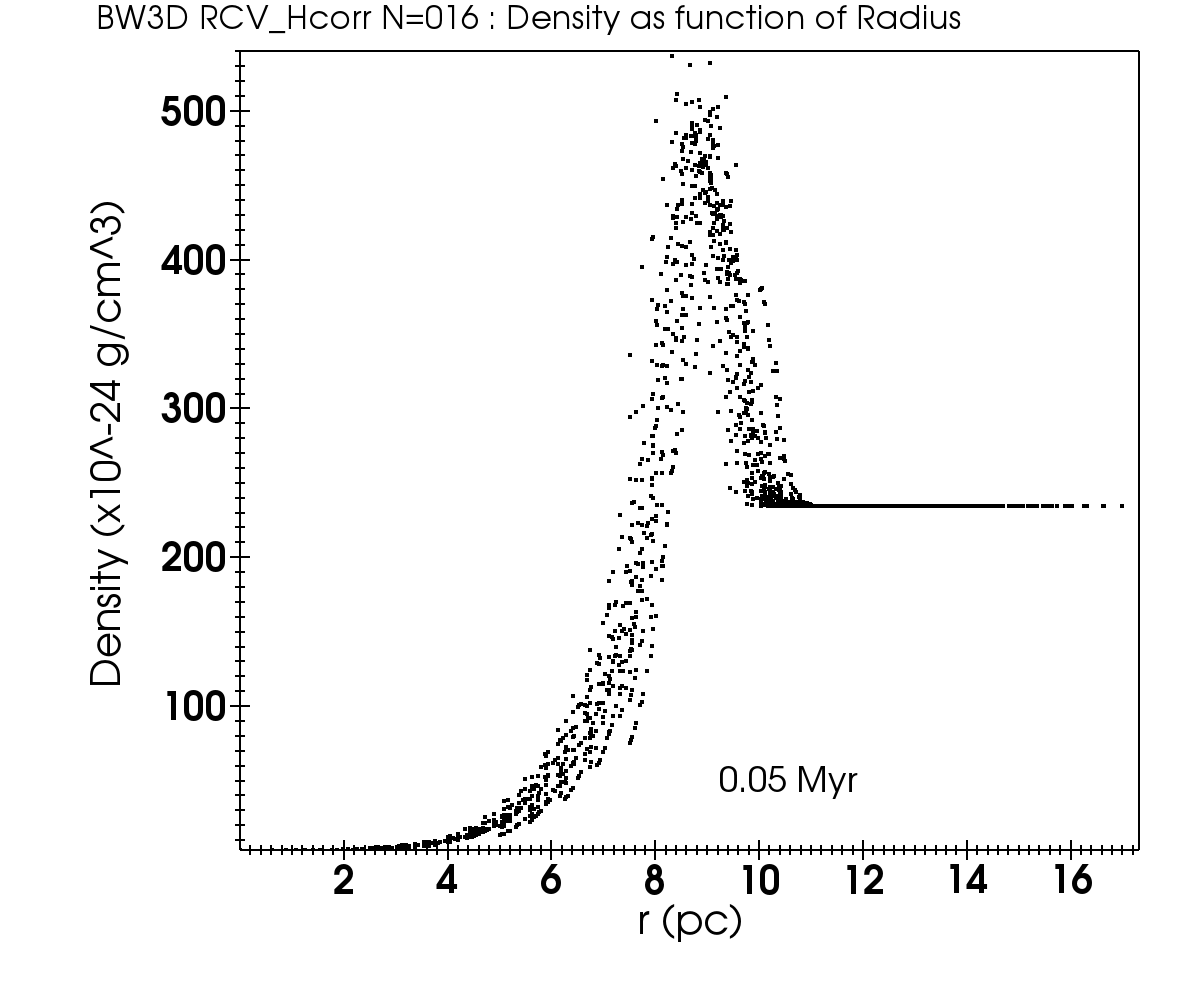
\includegraphics[width=0.32\textwidth]{figs/Density_BWcrt3Dpll_Octant_NR016_RCV_Hcorr_011.png}
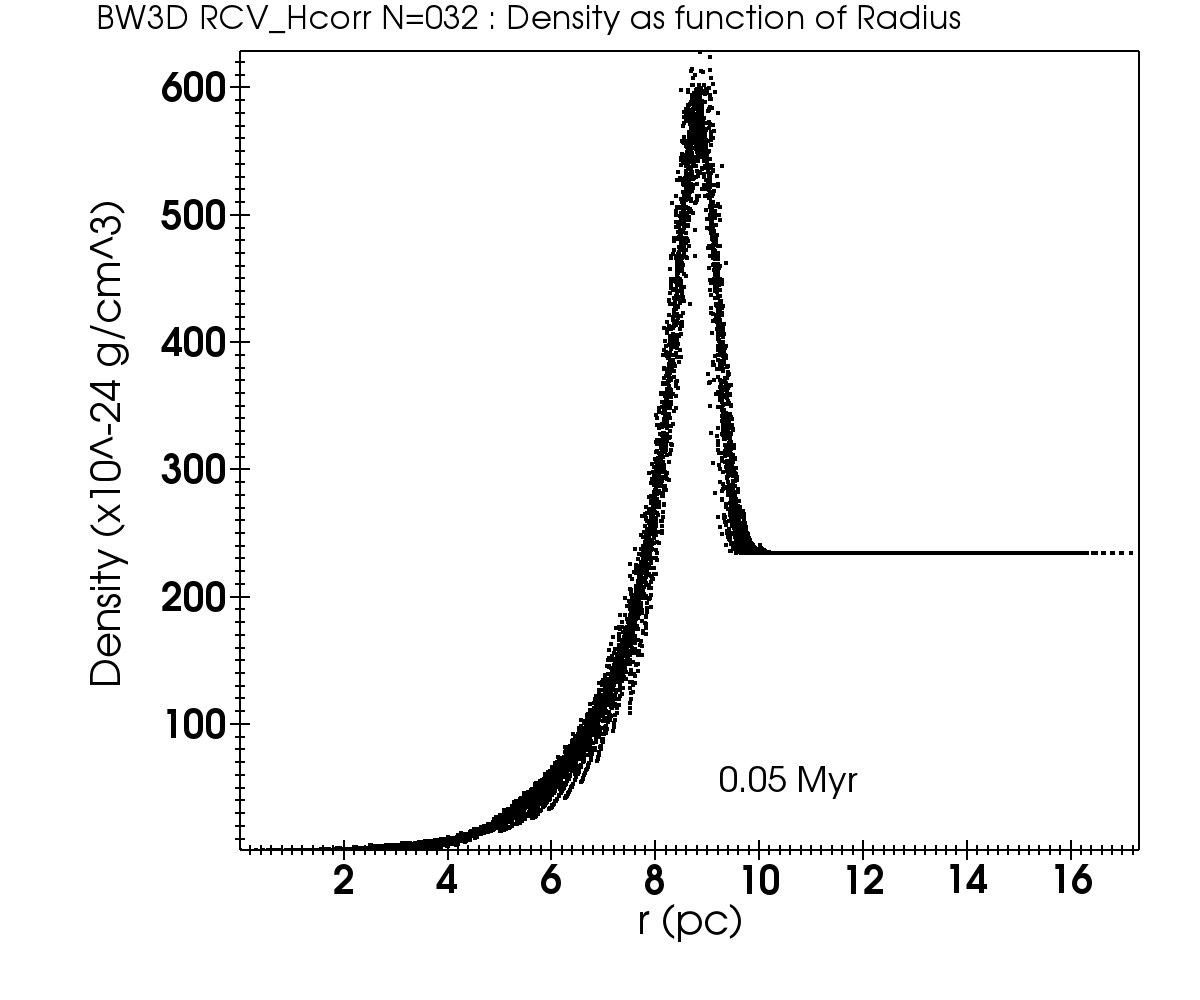
\includegraphics[width=0.32\textwidth]{figs/Density_BWcrt3Dpll_Octant_NR032_RCV_Hcorr_011.png}
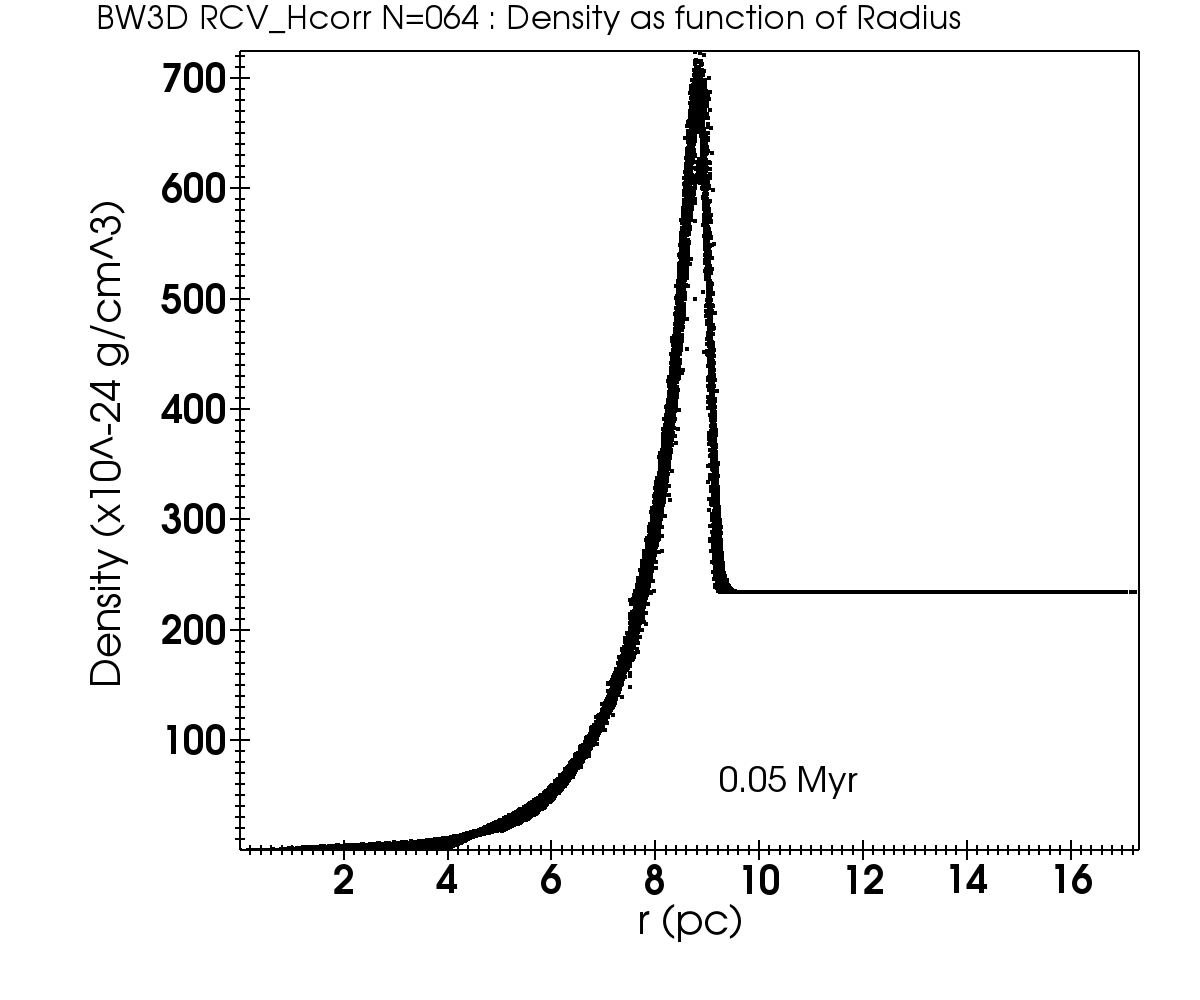
\includegraphics[width=0.32\textwidth]{figs/Density_BWcrt3Dpll_Octant_NR064_RCV_Hcorr_011.png}
\caption{
  Scatter plot of density against radius for a 3D adiabatic blastwave.
  The left-hand panel shows the result with $16^3$ grid zones, the centre panel with $32^3$ zones, and the right-hand panel with $64^3$ zones.
  All plots are for an evolutionary time of 0.05\,Myr.
  The test parameters are discussed in the text (sec.~\ref{sec:test:bw3d})
    }
\label{fig:bw3d_hd_adi_n032}
\end{figure}

\subsubsection{Unused parameters that are available for experimentation}
Magnetic field can be specified by the parameters \lstinline|BWmagfieldX, BWmagfieldY, BWmagfieldZ|, but note that this will not work with simple reflecting boundary conditions for a single octant.

Additionally a second ISM region can be specified, as a slab located at $x>x_0$, where $x_0$ is the interface coordinate (in cm) specified by the parameter \lstinline|BW_interface|.
Density, pressure, velocity can be set by parameters, \lstinline|BW_amb2_RO|, \lstinline|BW_amb2_PG|, \lstinline|BW_amb2_VX|, \lstinline|BW_amb2_VY|, and \lstinline|BW_amb2_VZ|, respectively.
\bibpunct{(}{)}{;}{a}{,}{,}

%%%%%%%%%%%%%%%%%%%%%%%%%%%%%%%%%%%%%%%%%%%%%%%%%%%%%%%%%%%%%%%%%%%%%
\section{StarBench test problems}
%%%%%%%%%%%%%%%%%%%%%%%%%%%%%%%%%%%%%%%%%%%%%%%%%%%%%%%%%%%%%%%%%%%%%

%%%%%%%%%%%%%%%%%%%%%%%%%%%%%%%%%%%%%%%%%%%%%%%%%%%%%%%%%%%%%%%%%%%%%
\section{Cosmological radiative transfer test problems}
%%%%%%%%%%%%%%%%%%%%%%%%%%%%%%%%%%%%%%%%%%%%%%%%%%%%%%%%%%%%%%%%%%%%%


\bibliographystyle{plainnat}
%\bibliographystyle{natbib}
\bibliography{./refs.bib}

\end{document}
